\subsection{Point  Class Reference}
\label{class_point}\index{Point@{Point}}
A point in a plane. 


{\tt \#include $<$point.h$>$}

Inheritance diagram for Point::\begin{figure}[H]
\begin{center}
\leavevmode
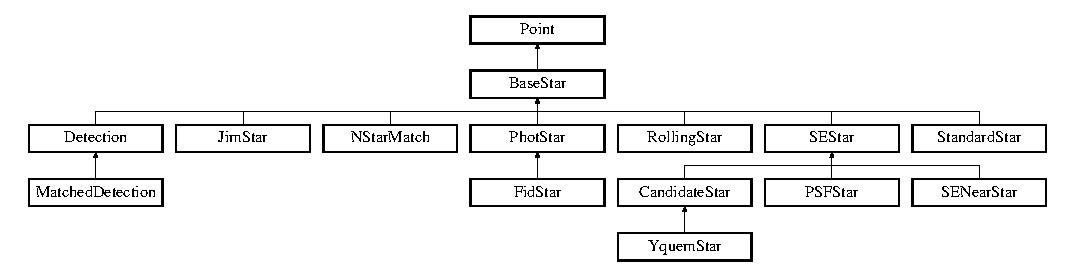
\includegraphics[height=3.27869cm]{class_point}
\end{center}
\end{figure}
\subsubsection*{Public Methods}
\begin{CompactItemize}
\item 
\index{Point@{Point}!Point@{Point}}\index{Point@{Point}!Point@{Point}}
{\bf Point} (const double \&xx=0, const double \&yy=0)\label{class_point_a0}

\begin{CompactList}\small\item\em \begin{CompactItemize}
\item 
contructor.\end{CompactItemize}
\item\end{CompactList}\item 
\index{Distance@{Distance}!Point@{Point}}\index{Point@{Point}!Distance@{Distance}}
double {\bf Distance} (const Point \&Other) const\label{class_point_a1}

\begin{CompactList}\small\item\em -.\item\end{CompactList}\item 
\index{Dist2@{Dist2}!Point@{Point}}\index{Point@{Point}!Dist2@{Dist2}}
double {\bf Dist2} (const Point \&Other) const\label{class_point_a2}

\begin{CompactList}\small\item\em distance squared to Other.\item\end{CompactList}\item 
\index{Apply@{Apply}!Point@{Point}}\index{Point@{Point}!Apply@{Apply}}
template$<$class Operator$>$ void {\bf Apply} (const Operator \&Op)\label{class_point_a3}

\begin{CompactList}\small\item\em Operator can be e.g. a {\bf Gtransfo} {\rm (p.\,\pageref{class_gtransfo})}.\item\end{CompactList}\item 
\index{operator+@{operator+}!Point@{Point}}\index{Point@{Point}!operator+@{operator+}}
Point {\bf operator+} (const Point \&Right) const\label{class_point_a4}

\begin{CompactList}\small\item\em Sum.\item\end{CompactList}\item 
\index{operator-@{operator-}!Point@{Point}}\index{Point@{Point}!operator-@{operator-}}
Point {\bf operator-} (const Point \&Right) const\label{class_point_a5}

\begin{CompactList}\small\item\em Difference.\item\end{CompactList}\item 
\index{dump@{dump}!Point@{Point}}\index{Point@{Point}!dump@{dump}}
virtual void {\bf dump} (ostream \&s=cout) const\label{class_point_a6}

\end{CompactItemize}
\subsubsection*{Public Attributes}
\begin{CompactItemize}
\item 
\index{x@{x}!Point@{Point}}\index{Point@{Point}!x@{x}}
double {\bf x}\label{class_point_m0}

\begin{CompactList}\small\item\em coordinate.\item\end{CompactList}\item 
\index{y@{y}!Point@{Point}}\index{Point@{Point}!y@{y}}
double {\bf y}\label{class_point_m1}

\begin{CompactList}\small\item\em coordinate.\item\end{CompactList}\end{CompactItemize}
\subsubsection*{Friends}
\begin{CompactItemize}
\item 
\index{operator<<@{operator$<$$<$}!Point@{Point}}\index{Point@{Point}!operator<<@{operator$<$$<$}}
ostream\& {\bf operator$<$$<$} (ostream \&stream, const Point \&point)\label{class_point_l0}

\begin{CompactList}\small\item\em -.\item\end{CompactList}\end{CompactItemize}


\subsubsection{Detailed Description}
A point in a plane.



The documentation for this class was generated from the following file:\begin{CompactItemize}
\item 
{\bf point.h}\end{CompactItemize}
